\documentclass[letterpaper,10pt,serif,draftclsnofoot,onecolumn,compsoc,titlepage]{IEEEtran}
\usepackage[margin=0.75in]{geometry} 
\usepackage{pdfpages} 
\usepackage{graphicx}  
\usepackage{caption} 
\usepackage{float}
\graphicspath{/images}
\usepackage{url}
\usepackage{setspace}
\usepackage{hyperref}
\usepackage{changepage}% http://ctan.org/pkg/changepage

  %pull in the necessary preamble matter for pygments output
\usepackage{fancyvrb}
\usepackage{color}
\usepackage[latin1]{inputenc}


\makeatletter
\def\PY@reset{\let\PY@it=\relax \let\PY@bf=\relax%
    \let\PY@ul=\relax \let\PY@tc=\relax%
    \let\PY@bc=\relax \let\PY@ff=\relax}
\def\PY@tok#1{\csname PY@tok@#1\endcsname}
\def\PY@toks#1+{\ifx\relax#1\empty\else%
    \PY@tok{#1}\expandafter\PY@toks\fi}
\def\PY@do#1{\PY@bc{\PY@tc{\PY@ul{%
    \PY@it{\PY@bf{\PY@ff{#1}}}}}}}
\def\PY#1#2{\PY@reset\PY@toks#1+\relax+\PY@do{#2}}

\expandafter\def\csname PY@tok@gd\endcsname{\def\PY@tc##1{\textcolor[rgb]{0.63,0.00,0.00}{##1}}}
\expandafter\def\csname PY@tok@gu\endcsname{\let\PY@bf=\textbf\def\PY@tc##1{\textcolor[rgb]{0.50,0.00,0.50}{##1}}}
\expandafter\def\csname PY@tok@gt\endcsname{\def\PY@tc##1{\textcolor[rgb]{0.00,0.25,0.82}{##1}}}
\expandafter\def\csname PY@tok@gs\endcsname{\let\PY@bf=\textbf}
\expandafter\def\csname PY@tok@gr\endcsname{\def\PY@tc##1{\textcolor[rgb]{1.00,0.00,0.00}{##1}}}
\expandafter\def\csname PY@tok@cm\endcsname{\let\PY@it=\textit\def\PY@tc##1{\textcolor[rgb]{0.25,0.50,0.50}{##1}}}
\expandafter\def\csname PY@tok@vg\endcsname{\def\PY@tc##1{\textcolor[rgb]{0.10,0.09,0.49}{##1}}}
\expandafter\def\csname PY@tok@m\endcsname{\def\PY@tc##1{\textcolor[rgb]{0.40,0.40,0.40}{##1}}}
\expandafter\def\csname PY@tok@mh\endcsname{\def\PY@tc##1{\textcolor[rgb]{0.40,0.40,0.40}{##1}}}
\expandafter\def\csname PY@tok@go\endcsname{\def\PY@tc##1{\textcolor[rgb]{0.50,0.50,0.50}{##1}}}
\expandafter\def\csname PY@tok@ge\endcsname{\let\PY@it=\textit}
\expandafter\def\csname PY@tok@vc\endcsname{\def\PY@tc##1{\textcolor[rgb]{0.10,0.09,0.49}{##1}}}
\expandafter\def\csname PY@tok@il\endcsname{\def\PY@tc##1{\textcolor[rgb]{0.40,0.40,0.40}{##1}}}
\expandafter\def\csname PY@tok@cs\endcsname{\let\PY@it=\textit\def\PY@tc##1{\textcolor[rgb]{0.25,0.50,0.50}{##1}}}
\expandafter\def\csname PY@tok@cp\endcsname{\def\PY@tc##1{\textcolor[rgb]{0.74,0.48,0.00}{##1}}}
\expandafter\def\csname PY@tok@gi\endcsname{\def\PY@tc##1{\textcolor[rgb]{0.00,0.63,0.00}{##1}}}
\expandafter\def\csname PY@tok@gh\endcsname{\let\PY@bf=\textbf\def\PY@tc##1{\textcolor[rgb]{0.00,0.00,0.50}{##1}}}
\expandafter\def\csname PY@tok@ni\endcsname{\let\PY@bf=\textbf\def\PY@tc##1{\textcolor[rgb]{0.60,0.60,0.60}{##1}}}
\expandafter\def\csname PY@tok@nl\endcsname{\def\PY@tc##1{\textcolor[rgb]{0.63,0.63,0.00}{##1}}}
\expandafter\def\csname PY@tok@nn\endcsname{\let\PY@bf=\textbf\def\PY@tc##1{\textcolor[rgb]{0.00,0.00,1.00}{##1}}}
\expandafter\def\csname PY@tok@no\endcsname{\def\PY@tc##1{\textcolor[rgb]{0.53,0.00,0.00}{##1}}}
\expandafter\def\csname PY@tok@na\endcsname{\def\PY@tc##1{\textcolor[rgb]{0.49,0.56,0.16}{##1}}}
\expandafter\def\csname PY@tok@nb\endcsname{\def\PY@tc##1{\textcolor[rgb]{0.00,0.50,0.00}{##1}}}
\expandafter\def\csname PY@tok@nc\endcsname{\let\PY@bf=\textbf\def\PY@tc##1{\textcolor[rgb]{0.00,0.00,1.00}{##1}}}
\expandafter\def\csname PY@tok@nd\endcsname{\def\PY@tc##1{\textcolor[rgb]{0.67,0.13,1.00}{##1}}}
\expandafter\def\csname PY@tok@ne\endcsname{\let\PY@bf=\textbf\def\PY@tc##1{\textcolor[rgb]{0.82,0.25,0.23}{##1}}}
\expandafter\def\csname PY@tok@nf\endcsname{\def\PY@tc##1{\textcolor[rgb]{0.00,0.00,1.00}{##1}}}
\expandafter\def\csname PY@tok@si\endcsname{\let\PY@bf=\textbf\def\PY@tc##1{\textcolor[rgb]{0.73,0.40,0.53}{##1}}}
\expandafter\def\csname PY@tok@s2\endcsname{\def\PY@tc##1{\textcolor[rgb]{0.73,0.13,0.13}{##1}}}
\expandafter\def\csname PY@tok@vi\endcsname{\def\PY@tc##1{\textcolor[rgb]{0.10,0.09,0.49}{##1}}}
\expandafter\def\csname PY@tok@nt\endcsname{\let\PY@bf=\textbf\def\PY@tc##1{\textcolor[rgb]{0.00,0.50,0.00}{##1}}}
\expandafter\def\csname PY@tok@nv\endcsname{\def\PY@tc##1{\textcolor[rgb]{0.10,0.09,0.49}{##1}}}
\expandafter\def\csname PY@tok@s1\endcsname{\def\PY@tc##1{\textcolor[rgb]{0.73,0.13,0.13}{##1}}}
\expandafter\def\csname PY@tok@sh\endcsname{\def\PY@tc##1{\textcolor[rgb]{0.73,0.13,0.13}{##1}}}
\expandafter\def\csname PY@tok@sc\endcsname{\def\PY@tc##1{\textcolor[rgb]{0.73,0.13,0.13}{##1}}}
\expandafter\def\csname PY@tok@sx\endcsname{\def\PY@tc##1{\textcolor[rgb]{0.00,0.50,0.00}{##1}}}
\expandafter\def\csname PY@tok@bp\endcsname{\def\PY@tc##1{\textcolor[rgb]{0.00,0.50,0.00}{##1}}}
\expandafter\def\csname PY@tok@c1\endcsname{\let\PY@it=\textit\def\PY@tc##1{\textcolor[rgb]{0.25,0.50,0.50}{##1}}}
\expandafter\def\csname PY@tok@kc\endcsname{\let\PY@bf=\textbf\def\PY@tc##1{\textcolor[rgb]{0.00,0.50,0.00}{##1}}}
\expandafter\def\csname PY@tok@c\endcsname{\let\PY@it=\textit\def\PY@tc##1{\textcolor[rgb]{0.25,0.50,0.50}{##1}}}
\expandafter\def\csname PY@tok@mf\endcsname{\def\PY@tc##1{\textcolor[rgb]{0.40,0.40,0.40}{##1}}}
\expandafter\def\csname PY@tok@err\endcsname{\def\PY@bc##1{\setlength{\fboxsep}{0pt}\fcolorbox[rgb]{1.00,0.00,0.00}{1,1,1}{\strut ##1}}}
\expandafter\def\csname PY@tok@kd\endcsname{\let\PY@bf=\textbf\def\PY@tc##1{\textcolor[rgb]{0.00,0.50,0.00}{##1}}}
\expandafter\def\csname PY@tok@ss\endcsname{\def\PY@tc##1{\textcolor[rgb]{0.10,0.09,0.49}{##1}}}
\expandafter\def\csname PY@tok@sr\endcsname{\def\PY@tc##1{\textcolor[rgb]{0.73,0.40,0.53}{##1}}}
\expandafter\def\csname PY@tok@mo\endcsname{\def\PY@tc##1{\textcolor[rgb]{0.40,0.40,0.40}{##1}}}
\expandafter\def\csname PY@tok@kn\endcsname{\let\PY@bf=\textbf\def\PY@tc##1{\textcolor[rgb]{0.00,0.50,0.00}{##1}}}
\expandafter\def\csname PY@tok@mi\endcsname{\def\PY@tc##1{\textcolor[rgb]{0.40,0.40,0.40}{##1}}}
\expandafter\def\csname PY@tok@gp\endcsname{\let\PY@bf=\textbf\def\PY@tc##1{\textcolor[rgb]{0.00,0.00,0.50}{##1}}}
\expandafter\def\csname PY@tok@o\endcsname{\def\PY@tc##1{\textcolor[rgb]{0.40,0.40,0.40}{##1}}}
\expandafter\def\csname PY@tok@kr\endcsname{\let\PY@bf=\textbf\def\PY@tc##1{\textcolor[rgb]{0.00,0.50,0.00}{##1}}}
\expandafter\def\csname PY@tok@s\endcsname{\def\PY@tc##1{\textcolor[rgb]{0.73,0.13,0.13}{##1}}}
\expandafter\def\csname PY@tok@kp\endcsname{\def\PY@tc##1{\textcolor[rgb]{0.00,0.50,0.00}{##1}}}
\expandafter\def\csname PY@tok@w\endcsname{\def\PY@tc##1{\textcolor[rgb]{0.73,0.73,0.73}{##1}}}
\expandafter\def\csname PY@tok@kt\endcsname{\def\PY@tc##1{\textcolor[rgb]{0.69,0.00,0.25}{##1}}}
\expandafter\def\csname PY@tok@ow\endcsname{\let\PY@bf=\textbf\def\PY@tc##1{\textcolor[rgb]{0.67,0.13,1.00}{##1}}}
\expandafter\def\csname PY@tok@sb\endcsname{\def\PY@tc##1{\textcolor[rgb]{0.73,0.13,0.13}{##1}}}
\expandafter\def\csname PY@tok@k\endcsname{\let\PY@bf=\textbf\def\PY@tc##1{\textcolor[rgb]{0.00,0.50,0.00}{##1}}}
\expandafter\def\csname PY@tok@se\endcsname{\let\PY@bf=\textbf\def\PY@tc##1{\textcolor[rgb]{0.73,0.40,0.13}{##1}}}
\expandafter\def\csname PY@tok@sd\endcsname{\let\PY@it=\textit\def\PY@tc##1{\textcolor[rgb]{0.73,0.13,0.13}{##1}}}

\def\PYZbs{\char`\\}
\def\PYZus{\char`\_}
\def\PYZob{\char`\{}
\def\PYZcb{\char`\}}
\def\PYZca{\char`\^}
\def\PYZam{\char`\&}
\def\PYZlt{\char`\<}
\def\PYZgt{\char`\>}
\def\PYZsh{\char`\#}
\def\PYZpc{\char`\%}
\def\PYZdl{\char`\$}
\def\PYZti{\char`\~}
% for compatibility with earlier versions
\def\PYZat{@}
\def\PYZlb{[}
\def\PYZrb{]}
\makeatother


%% The following metadata will show up in the PDF properties
\usepackage{listings}
\usepackage{color}
\definecolor{lightgray}{rgb}{0.95, 0.95, 0.95}
\definecolor{darkgray}{rgb}{0.4, 0.4, 0.4}
\definecolor{purple}{rgb}{0.65, 0.12, 0.82}
\definecolor{ocherCode}{rgb}{1, 0.5, 0} % #FF7F00 -> rgb(239, 169, 0)
\definecolor{blueCode}{rgb}{0, 0, 0.93} % #0000EE -> rgb(0, 0, 238)
\definecolor{greenCode}{rgb}{0, 0.6, 0} % #009900 -> rgb(0, 153, 0) 
\usepackage{upquote}
\usepackage{listings}
\makeatletter
\lstdefinelanguage{HTML5}{
sensitive=true,
keywords={%
% JavaScript
ng-src, ng-repeat, typeof, new, true, false, catch, function, return, null, catch, switch, var, if, in, while, do, else, case, break,
% HTML
html, title, meta, style, head, body, script, canvas,
% CSS
border:, transform:, -moz-transform:, transition-duration:, transition-property:,
transition-timing-function:
},
% http://texblog.org/tag/otherkeywords/
otherkeywords={<, >, \/},   
ndkeywords={class, export, boolean, throw, implements, import, this},   
comment=[l]{//}, 
% morecomment=[s][keywordstyle]{<}{>},  
morecomment=[s]{/*}{*/},
morecomment=[s]{<!}{>},
morestring=[b]',
morestring=[b]",    
alsoletter={-},
alsodigit={:}
}
\lstset{%
% Basic design
backgroundcolor=\color{lightgray},
basicstyle={\small\ttfamily},   
frame=l,
% Line numbers
xleftmargin={0.75cm},
numbers=left,
stepnumber=1,
firstnumber=1,
numberfirstline=true,
% Code design
identifierstyle=\color{black},
keywordstyle=\color{blue}\bfseries,
ndkeywordstyle=\color{greenCode}\bfseries,
stringstyle=\color{ocherCode}\ttfamily,
commentstyle=\color{darkgray}\ttfamily, 
% Code 
tabsize=1,
showtabs=false,
showspaces=false,
showstringspaces=false,
extendedchars=true,
breaklines=true
}
\lstdefinelanguage{JavaScript}{
  keywords={typeof, new, true, false, catch, function, return, null, catch, switch, var, if, in, while, do, else, case, break},
  keywordstyle=\color{blue}\bfseries,
  ndkeywords={class, export, boolean, throw, implements, import, this},
  ndkeywordstyle=\color{darkgray}\bfseries,
  identifierstyle=\color{black},
  sensitive=false,
  comment=[l]{//},
  morecomment=[s]{/*}{*/},
  commentstyle=\color{purple}\ttfamily,
  stringstyle=\color{red}\ttfamily,
  morestring=[b]',
  morestring=[b]"
} 

%% The following metadata will show up in the PDF properties
\hypersetup{
   colorlinks = true,
   citecolor = black,
   linkcolor = black,
   urlcolor = black,
   breaklinks = true,
   pdfauthor = {Daniel Schroeder, Aubrey Thenell, Parker Bruni},
   pdfkeywords = {CS462 Senior Project Progress Report},
   pdftitle = {CS462 Winter Midterm Progress Report},
   pdfsubject = {CS462 Winter Midterm Progress Report},
   pdfpagemode = UseNone
}
\def \CapstoneTeamName{The Dream Team}
\def \CapstoneTeamNumber{57}
\def \GroupMemberOne{Daniel Schroeder}
\def \GroupMemberTwo{Aubrey Thenell}
\def \GroupMemberThree{Parker Bruni}
\def \CapstoneProjectName{A Scalable Web Application Framework for Monitoring Energy Usage on Campus  }
\def \CapstoneSponsorCompany{Oregon State Office of Sustainability}
\def \CapstoneSponsorPerson{Jack Woods}

% 2. Uncomment the appropriate line below so that the document type works
 \def \DocType{		%Problem Statement
		 %Requirements Document
		 %Technology Review
		 %Design Document
		 Winter 2018 Midterm Progress Report
		 }
	   
 \newcommand{\NameSigPair}[1]{\par
 \makebox[2.75in][r]{#1} \hfil 	\makebox[3.25in]{\makebox[2.25in]{\hrulefill} \hfill		\makebox[.75in]{\hrulefill}}
 \par\vspace{-12pt} \textit{\tiny\noindent
 \makebox[2.75in]{} \hfil		\makebox[3.25in]{\makebox[2.25in][r]{Signature} \hfill	\makebox[.75in][r]{Date}}}}
 % 3. If the document is not to be signed, uncomment the RENEWcommand below
 %\renewcommand{\NameSigPair}[1]{#1}
 
 %%%%%%%%%%%%%%%%%%%%%%%%%%%%%%%%%%%%%%%
 \title{Winter 2018 Progress Report for: \linebreak Scalable Web Application Framework for Monitoring Energy Usage on Campus}
 \author{Daniel Schroeder, Aubrey Thenell, Parker Bruni}
 \date{\today}
 
 \begin{document}
 \maketitle
 \vspace{2cm}
 \begin{center}
 \noindent \textbf{Abstract} \\
			 \indent 
 \end{center}         
 
 \newpage
 \pagenumbering{arabic}
\tableofcontents
\newpage

\section{Introduction}
\subsection{Purpose}
\subsection{Scope}
\subsection{Overview}
This document provides a recap of the progress made on our project during the Winter 2018 term. \\
Update this section \\ 
\section{Contributor: Daniel Schroeder} 
\subsection{Describe where you are currently on the project}
Since the end of fall term, I have implemented 3/4 main components of the application with back-end functionality and data-binding working. These components include Buildings, Blocks, and Dashboards. In addition, I generated important mongoose.js and AngularJS code for repeated iterations and element generation of User-stored data and saving documents created by the user. I got Google oAuth working on the application with user objects stored by Google API tokens and create user sessions throughout the application with passport.js. 
\subsubsection{Buildings}
The building components are data models stored in the database with attributes like name, type, id, serial, and array of data points. To generate components that display these buildings, we needed to store the data along with building images and create a page to list them in a logical way. To accomplish this, I scraped the internet for a photo of each building we needed in the application and stored them in our assets folder with a name that corresponds to the building object name that is stored in the database. On the ``/buildings'' page, a building service retrieves all the building objects from the database which are used as the data model for an AngularJS ``ng-repeat'' directive to generate identical components. The outcome is a precise, columned list of card components that link to specific building pages and display the object's name and photo. 
\begin{figure}[H]
  \centering
  \includegraphics[width=17cm]{images/buildings.eps}
  \caption{A screen shot of the building components being listed by the ng-repeat AngularJS directive.}
\end{figure}
Some clever code I used for the building components includes a regular expression used to parse the building name and convert it to the image address for the photo. As shown below, each building component has an ``\textless img\textgreater'' tag inside its card which calls a controller function ``getImageAddress''. This function executes a regular expression in the controller based on the building object that gets passed in from the view.
\begin{lstlisting}[language=HTML5]
<!--buildings.html-->
<div class="card-body ml-3">
  <h5 class="card-title">{{building.name}}</h5>
  <div class="rounded mx-auto mt-3" style="height: 100px; width: 100px;">
      <img class="rounded" ng-src="{{getImageAddress(building)}}" alt="">
  </div>
  <p class="mt-3"><b>Type: </b>{{building.building_type}}</p>
  <p><b>Meter ID: </b>{{building.meter_id}}</p>
  <a ng-click="viewBuilding(building)" href="#viewBuilding" class="...">View</a>
</div>
\end{lstlisting}
\begin{lstlisting}[language=JavaScript]
//building-controller.js
$scope.getImageAddress = function(building) {
  return "../assets/buildings/"+building.name.replace(/\s+/g, '-').toLowerCase()+".jpg";
};
\end{lstlisting}
These building components will be publicly viewable and each building card has a ``view'' button which links to the individualized building page. These individual pages will contain (they are not yet completed) information about the building like photos, name, and type, and a personalized report for the specific building with consumption information and charts.
\subsubsection{Blocks}
\begin{figure}[H]
  \centering
  \includegraphics[width=17cm]{images/block-example.eps}
  \caption{A screen shot of a block component created by the user with three building objects.}
\end{figure}
The block components I built are the ``building blocks'' of user dashboards and the hub for user created graphs/reports. A Block object contains an array of buildings, a graph, and a name. A block generates a specific type of graph based on the building(s) selected and the type of graph the user selected. The D3.js visualizations have not been implemented yet, but each block will retrieve and parse the data for each building it stored in its building array and generate a D3.js visualization. These graphs can range from simple consumption over time line graphs, to comparison graphs between multiple buildings.\\

\noindent To implement these components, I had to create a model schema, build a create form page, and design the UI. Additionally, I needed to create controller functions and AngularJS services to handle data creation, retrieval, and storing. We wanted a way to keep track of which blocks were created by which users, so in addition to a Blocks table in the database, each user has an array of type Block within their user object that gets pushed to and pulled from on creation or deletion. This architecture makes data retrieval much simpler for a few reasons:
\begin{itemize}
  \item Do not need to iterate through the entire Block table when retrieving user blocks.
  \item Mongoose.js has a .populate function that populates sub-documents referenced by other documents. 
  \item Block retrieval service can be user-specific.
\end{itemize}
To elaborate more on this style of NoSQL database management, I will show our User and Block schemas and explain how I implemented the storing and retrieval.
\begin{lstlisting}[language=JavaScript]
var blockSchema = mongoose.Schema({
  name         : String,
  created_by   : {type:mongoose.Schema.ObjectId, ref: 'User'},
  building     : [{type:mongoose.Schema.ObjectId, ref: 'Building'}],
  chart        : String,
  variable     : String
});

var userSchema = mongoose.Schema({
  google           : {
      id           : String,
      token        : String,
      email        : String,
      name         : String
  },
  blocks           : [{type:mongoose.Schema.ObjectId, ref: 'Block'}],
  dashboards       : [{type:mongoose.Schema.ObjectId, ref: 'Dashboard'}]
});
\end{lstlisting}
The User schema defines a User as having an array of block objects and an array of Dashboard objects (defined by the ``[ ]'' in the attribute definition). One thing to notice is the mongoose syntax for referencing another schema with the definition mongoose.Schema.ObjectId. This is the mongoose equivalent of setting a foreign key. When we push a document to the User.block array, the Block.\_id will be stored in this block array, effectively creating what mongoose likes to call a sub-document. More explicitly: ``Sub-documents are documents embedded in other documents. In Mongoose, this means you can nest schemas in other schemas''\cite{mongoose}. Creating a ``relational database'' like this with NoSQL allowed me to generate simple queries in our API route handlers that find a User, populate all the referencing sub-documents, and return the resulting JSON back to the controller. From here, we are able to store references to buildings in the block objects, references to blocks in the dashboard objects, and only populate data when we need it in the application. 
\subsubsection{Dashboards} 
The dashboard components are the last thing I worked on and are not yet fully complete. What I wanted to get finished before the midterm milestone was creating dashboards and storing dashboards, which I accomplished. There is a ``create-dashboard'' form that data-binds all user blocks to a drop down menu using AngularJS directive ``ng-options'' so that a user is able select which blocks they want to include in the dashboard. In addition, the form has a text-box for a dashboard name and a multi-line text-box for a description attribute, all of which are gathered up by the dashboard controller and passed to an API route-handler that stores the new Dashboard object in the database.\\

\noindent The dashboards followed the same suit as the Block objects as they were stored in an array within the creating User's object as well as in their own table in the database. This produced some difficulties when querying updates and deletes as we had to ensure that both references were updated for a successful return. I still have to implement the ``view dashboard'' feature which will consist of iterating over each Block stored in the Dashboard and rending its content/graphs in a sequential order. Our dashboards are essentially the same as the ``view blocks'' page with block components listed one after the other, except it contains a user-defined subset of blocks for a specific analysis. 
\subsubsection{Important Data-Binding Code}
Throughout the application, I have implemented AngularJS directives/services to retrieve and render data to the screen. Here are a few specific code samples I want to share that were either duplicated and used on multiple pages, or I just thought they were impressive implementations.\\

\noindent First is the ``ng-repeat'' directive we use for buildings, dashboards, and blocks to iterate through a data set and produce multiple HTML elements ``for-each'' object in the set. This implementation requires a data set to be provided by the controller and an HTML template to be repeated. A particularly interesting example of this was a nested ``ng-repeat'' used to display all the user blocks, and all the buildings inside each block. 
\begin{lstlisting}[language=HTML5]
<!--blocks.html-->
<div ng-controller="blockController">
<div class="card mb-3" style="width: 90%;" ng-repeat="block in userBlocks">
  <div class="card-header h-100">
    <div class="h-100 d-inline-flex">
      <span class=" align-middle ">
        {{block.name}}
      </span>
    </div>
    ...
    <h3>Buildings:</h3>
    <ul>
      <li ng-repeat="building in block.building">
        {{building.name}}
      </li>
    </ul>
  ...
\end{lstlisting}
On line 13 of the listing, we see that the data model being repeated is being taken from the block object returned by the ``ng-repeat'' directive on line 3. This essentially allows ``double for-loop'' style data-binding to occur in the view and which displays all the necessary information to the user with only a couple lines of code.\\

\noindent Next, I wanted to share how I was able to create a functioning relation database with MongoDB and mongoose.js using sub-documents and the mongoose.js ``.populate()'' function in our API. In order to keep our object sizes small, we only store references (ObjectId's) into model arrays like Block.buildings or User.dashboards. In order to retrieve this data and render it for the user, we need to dereference the ObjectId's in the back-end before returning the object to the controller. To do this, we have to populate the sub-documents so mongoose can retrieve the actual objects from the database and return all the necessary information. I'm going to share the API query for achieving this for the same situation as the nested ``ng-repeat'' above, as it also required a nested ``.populate()'' call to dereference sub-documents and sub-sub-documents.
\begin{lstlisting}[language=JavaScript]
app.get('/api/getUserBlocks', function(req, res) {
  User.findOne({_id : req.user._id})
    .populate({ path: 'blocks',
        populate: {path: 'building'}
    })
    .exec(function (err, user) {
      if (err) return handleError(err);
      res.json(user.blocks); });
});
\end{lstlisting}
As seen on line 4 of the listing, we call a populate from within a populate which dereferences the sub-sub-documents ``building'' that are being referenced by the sub-document ``blocks.'' This ensures that we have access to the building names and types when returning the user blocks to the controller. If we did not populate these sub-documents, the query would only return the ObjectId's with no relevant information for display.\\
\noindent 
\subsubsection{Authentication}
\begin{figure}[H]
  \centering
  \includegraphics[width=17cm]{images/login.eps}
  \caption{A screen shot of the login page that uses Google oAuth to authenticate users.}
\end{figure}
In addition to component functionality and implementation, I was able to get Google oAuth2.0 authentication to work with our application and authenticate users based on Google token. I had our client (Jack Woods) generate a Google API key under an Office of Sustainability Gmail account and used that API key to set up our authentication protocol. I used passport.js as an authentication middleware which handles most of the session authentication and oAuth functionality. I stored the token that Google's API returned in the user object which is what our application uses instead of a password. The next steps to take for authentication is limiting access to certain pages depending on user role and generating ``per-page'' authentication middleware to track users across pages.
\subsubsection{Other Features I Accomplished}
Despite the big features mentioned above, other tasks I accomplished since last term are:
\begin{itemize}
  \item Stored all sensitive information as ENV variables accessible through ``dotenv'' npm library.
  \item Created User, Block, Dashboard, and Building services to call API route handlers and access data.
  \item Formatted ``Our Team'' section into tri-column sections with colored job-titles and blank avatar images.
  \item Generated angular routes in the core.js file to create SPA (single page application) protocols for linking and navigation.
  \item Built the pop-out story menu in sidebar.
  \item Built side navigation.
  \item Added all building images in assets folder.
  \item Created highlighting effects and border removal AJAX functionality for navigation selection.
  \item Created the dynamic population of ``selected buildings'' in create block form. 
  \item Created the dynamic population of ``selected blocks'' in create dashboard form. 
  \item Implemented delete block functionality (button, back-end query, and redirect).
  \item Implemented delete dashboard functionality (button, back-end query, and redirect).
  \item Generated mock-up table for data records in individual building pages.
  \item Created a database configuration file to generate all the buildings with example data.
\end{itemize}
\subsection{Describe what you have left to do}
Some things I still need to accomplish:
\begin{itemize}
  \item Implement story functionality.
  \item Create ``edit'' pages for block, dashboard, and story components.
  \item Filter settings on buildings page.
  \item Limit viewable content based on user roles and authentication.
  \item Make public vs. private flag on user items.
  \item Create public facing application distinction.
  \item Generate D3.js templates for different graph types.
\end{itemize}
\section{Contributor: Aubrey Thenell}
\subsection{Describe where you are currently on the project}
\subsection{Describe what you have left to do}
\subsection{Describe any problems that have impeded your progress, with any solutions}
\subsection{Include particularly interesting pieces of code}
\subsection{Images of our Project} 

\section{Contributor: Parker Bruni}
\subsection{Describe where you are currently on the project}
	At the end of Fall term we had completed our design document and got approval from our client that our design was acceptable and we began work during winter break.
	So far, I have been assigned to mainly handle the overall look, feel, and front-end design of our project. Progress towards making our application display as a clean and intuitive 
	interface has gone well, without many problems or issues along the way. We ultimately want our application to provide utility, so most of my focus has been for that. I have
	opted to avoid using flashy or dazzling UI animations or themes to avoid confusion by the user, but the application still needed a clean and modern feel for the user to be 
	comfortable when working. Our color scheme is representative of this, using mostly neutral colors with a few bright colors such as OSU orange as trim to add a little life 
	to the interface. 
	
	\subsubsection{Fonts and CSS Classes}
	The font of our application utilizes a directory of Oregon State Marketing approved font files of type ``.otf'', ``.woff'', and ``.woff2.'' The font family that 
	these files include are ``rufina-stencil-regular'' for the main heading of the application and ``Stratum2'' for other headers. Our body paragraphs will utilize ``Open-Sans''
	for paragraph elements and elements of lesser importance, as per OSU Marketing guidelines. These font files 
	are implemented within our CSS file so that they may be accessed by the HTML elements of our page directly from the CSS file. This is demonstrated in the code below
	
\begin{lstlisting}[caption={CSS Implementation} language=CSS]
@font-face {
  font-family: 'rufina-stencil-regular';
  src: url('assets/fonts/rufina-stencil-regular.otf') format('opentype'),
       url('assets/fonts/rufina-stencil-regular.woff') format('opentype'),
       url('assets/fonts/rufina-stencil-regular.woff2') format('opentype');
}

.rufina-stencil-regular {
	font-family: 'rufina-stencil-regular';
}
\end{lstlisting}
\begin{lstlisting}[caption={HTML Implementation} language=HTML]
<h1 class="rufina-stencil-regular m-0">Oregon State University</h1>
\end{lstlisting}

	As you can see from the code, the HTML element is assigned a class which has the desired font associated with it. Each font that we have available can be 
	implemented in an element by adding the class name, essentially functioning as an ``argument'' by which that element should behave. In this way, we can simply
	add arguments to our elements via class names to give it certain CSS attributes without having to hard code the CSS style directly into the element. This method is used in our application for many
	different types desired CSS attributes, such as font, alignment, background-color, position, etc. It allows us great control when customizing CSS attributes without 
	needing to add a specific class for every element. Many of our HTML elements use this technique but utilizing Bootstrap libraries as well, such as generating CSS for 
	our login button element. 
	\subsubsection{Top Navigation}
	Our application top navigation bar has various elements within it. Specifically, in order from left to right, the top navigation bar contains a application logo, 
	selectable elements that redirect the user to our ``Home'', ``About'', and ``Contacts'' page, our applications title, and our login button. The top navigation bar 
	is a fixed size and position on the page and will exist on all pages until the application is put into presentation mode. It's background color is a very dark gray to achieve
	a modern look and contrast with the white body of our page and the lighter gray side navigation bar. 
	
	\subsubsection{Logo}
    \begin{figure}[H]
      \centering
      
\includegraphics[width=17cm]{images/logo.eps}
      \caption{Our current logo for the application, located in the left-most region of the top nav.}
    \end{figure}
  In the current version of our application, our logo has been decided by our client to be an Oregon State official logo. The logo was requested and has been provided for us 
  in the format of a ``.svg'' file by our client. Having the logo as a scalable vector graphics file will allow the logo adjust to the size of its parent element without loss 
  of resolution or quality if the parent element is to scale up. We do not necessarily have to worry about this as the parent element of our logo will be a fixed
  size because our top navigation is a fixed size. I have requested to our client that we get a logo that is tailored to our website by a member of the OSU marketing
  team because it would be much more fitting that our logo includes our application name. Another reason to get a customized logo is because the font of the logo contains
  black letters which blend in with the dark background of our top navigation bar.
		
		\subsubsection{Selectable Elements}
		The top navigation bar also includes selectable elements so the user can navigate the pages. The elements text highlights on hover but perform no special UI functions
		when clicked. 
			\subsubsection{Home}
			The first element is the ``Home'' tab. When this tab is clicked, the user is redirected to the homepage of our application. This page contains the title of our 
			application as well as a Google Maps API angular.js implementation. The map will contain a KML layer of all of the buildings with metering systems installed, and 
			when a user selects one of these buildings from the map, they will be redirected to that buildings energy dashboard page. Ideally, this homepage will be used
			mostly by the public where our application will be displayed on a monitor located in buildings on campus.
			\subsubsection{About}
			Our about page contains information about the goal of the application, the history of the Office of Sustainability, the mission of of the Office of Sustainability,
			and links to the social media websites related to the Office of Sustainability.
			\subsubsection{Contact}
			Our about page contains the basic contact information of a select few OSU Office of Sustainability members as well as the developers of the application.
			
	\subsubsection{Side Navigation}
	The side navigation was implemented by another member of our team, but I have contributed to the overall look and feel of the side navigation. I have added small
	animations that indicate to the user which tab has been selected. The first animation fluidly indents the title of the tab when it is being displayed by the 
	body of our page. This is achieved by increasing the ``padding-left'' of the element from 0px to 6px over the course of 0.2 seconds. The second animation changes the 
	left side border from dark gray to OSU orange over the course of 0.2 seconds. The code and images below demonstrate this effect.
	
\begin{figure}[H]
  \centering
  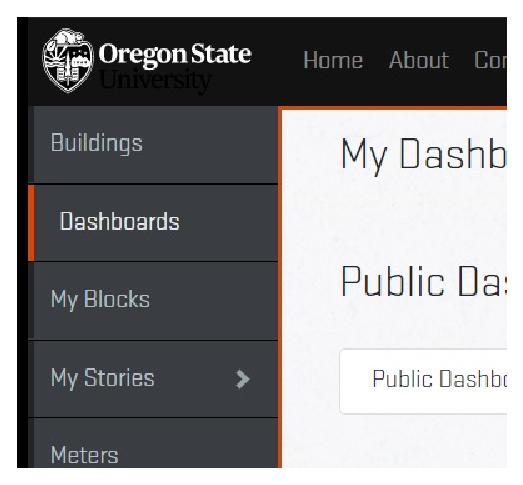
\includegraphics[width=17cm]{images/side-nav-css.eps}
  \caption{Side navigation tab selection CSS (orange border and text indent).}
\end{figure}
	
\begin{lstlisting}[caption={CSS Implementation} language=CSS]
.custom-nav-item div{
    border-left: 4px solid;
	
}
.active-nav-item div{
    border-left: 4px solid #DC4405;
    -webkit-transition: all 0.3s ease-in-out 0s;
    transition: all 0.3s ease-in-out 0s;
}
.active-nav-item .custom-nav-link{
    padding-left: 6px;
	-webkit-transition: all 0.2s ease-in-out 0s;
    transition: all 0.2s ease-in-out 0s;
}
\end{lstlisting}
	
	These combined CSS animations give modern feel yet clear indication of which tab is selected.
	
\subsection{Describe what you have left to do}
Some things that I still need to accomplish:
\begin{itemize}
  \item Add KML layer to Google Maps API
  \item Change body font
  \item Adjust top nav title design
  \item Obtain customized logo
  \item Format Buildings page CSS and UI
  \item Format Dashboards page CSS and UI
  \item Format My Stories page CSS and UI
  \item Format Meters page CSS and UI
  \item Format Settings page CSS and UI
  \item Add ``Presentation Mode'' to remove navigation bars and create a more presentable view of application for public access
  \item Create an official color scheme with set hex color values
\end{itemize}
\subsection{Describe any problems that have impeded your progress, with any solutions}
One problem that I had was with our Google Maps API. I had followed a tutorial for adding the Google Maps API but the map was not functioning. I thought this could 
be because I did not have a valid Map ``key'' but I tried many different valid keys and this was not the case. I transferred the code that I was using from our application
to a simple test implementation and the code worked. For whatever reason, the format of our application was breaking the map. This could be due to our page being a 
MEAN stack single page application. My solution was to simply look for tutorials on how to implement a Google Map on this style of application. I found a good example and 
adjusted the code to fit our website. Essentially, I needed to make a controller for this API and eventually the map was functional and displaying properly.

\subsection{Include particularly interesting pieces of code}
\subsection{Images of our Project} 


\newpage
\bibliographystyle{ieeetr}
\bibliography{refs.bib}
\end{document}
